Em muitas pesquisas, estamos interessados no efeito do tratamento em mais de uma variável. Nesses casos, é comum com que o pesquisador planeje corrigir o teste por múltiplas hipóteses. Quando estamos testando hipóteses para múltiplas variáveis diferentes, a probabilidade de rejeitarmos uma hipótese nula verdadeira para pelo menos uma das variáveis é maior do que nível de significância, $\alpha$, utilizado em cada um dos testes. Por exemplo, se testarmos 10 hipóteses independentes ao nível de significância de 5\%, então pelo menos uma hipótese nula verdadeira será rejeitada com probabilidade de 40\%.\footnote{A probabilidade de nenhuma das hipóteses nulas verdadeiras serem rejeitadas é de $(1-0.05)^{10}$. Portanto, a probabilidade de pelo menos uma hipótese nula verdadeira ser rejeitada é de $1 - (1-0.05)^{10} \approx 40\%$.}

Um jeito comum de corrigirmos por hipóteses múltiplas é separando as variáveis de interesse em diferentes famílias. A tabela \ref{primary_outcomes} é um exemplo de separação para nosso exemplo empírico. A \textbf{Família I} se refere às variáveis de mercado de trabalho, enquanto que a \textbf{Família II} se refere às variáveis de desempenho escolar. Ao agruparmos por famílias, estamos interessados em ver se o efeito do tratamento numa família de variáveis é significantemente diferente de zero (veja Anderson, 2008).


\begin{table}[h]
\centering
\caption{\sc Famílias de Variáveis de Interesse}
\label{primary_outcomes}
\resizebox{\textwidth}{!}{\begin{tabular}{lll}
\toprule
 & \textbf{Tipo} & \textbf{Variáveis} \\
 \midrule
  \multirow{2}{*}{\textbf{Família I.}} & \multirow{2}{*}{Mercado de Trabalho}   & \textbf{1.} Está empregado ou não \\
  & &\textbf{2.} Formal ou informal \\
    \midrule

  \multirow{3}{*}{\textbf{Família II.} } & \multirow{3}{*}{Desempenho Escolar} & \parbox{7cm}{\textbf{3.} Nota na prova} \\
             & &\textbf{4.} Frequência\\
             & &\textbf{5.} Está matriculado ou não\\
\bottomrule
\end{tabular}}

\end{table}

Para levarmos o teste de múltiplas hipóteses em consideração quando estamos calculando poder, podemos corrigir o nível de significância que estamos utilizando no cálculo do MDE. Um método comum e prático é ajustar o nível de significância para o tamanho de cada família, utilizando a correção de \v{S}idák:
\begin{equation}
    \alpha_h = 1 - (1-0.05)^{\frac{1}{h}}
\end{equation}

\noindent em que $h$ é o número de variáveis dentro da família que estamos querendo testar a hipótese. Note que se $h = 1$, temos o mesmo $\alpha = 0.05$. Ao aumentarmos $h$, o nível de significância que iremos utilizar diminui, fazendo com que a probabilidade de rejeitarmos pelo menos uma hipótese nula verdadeira seja de 5\%.\footnote{Isso acontece caso as hipóteses sejam independentes. Caso elas tenham correlação positiva, o teste é conservador e, caso a correlação seja negativa, o teste é inválido. Um jeito comum de evitar correlação negativa entre os teste é mudar o sinal das variáveis para que a direção positiva delas indique uma ``melhoria'' na variável (veja \citealp{anderson2008}).} Existem outros métodos que podem ser utilizados, como a correção de Bonferroni ou a correção de Holm (veja \citealp{anderson2008}), porém iremos utilizar apenas a correção de \v{S}idák nos nossos exemplos empíricos na próxima seção.

\section{Praticando: Fórmula Analítica}

Nesta seção, iremos calcular o MDE para o caso de múltiplas hipóteses apenas utilizando a fórmula analítica. Aqui, estamos levando em consideração apenas a correção do nível de significância, mas não entraremos em detalhes a respeito do teste de múltiplas hipóteses.\footnote{Existem várias maneiras de testarmos múltiplas hipóteses conjuntamente. Ao termos acesso aos dados, além de corrigirmos o nível de significância, temos que nos preocupar em como agregar as variáveis para o teste conjunto. Veja \cite{anderson2008} para mais detalhes deste assunto.}

Primeiramente, iremos limpar o ambiente de trabalho, carregar os pacotes necessários e definir os parâmetros que estarão fixos no cálculo do MDE.

\begin{boxH}
\begin{lstlisting}[language = R]
# Limpar o ambiente 
rm(list=ls())

# Carregando pacotes necessários
library(tidyverse)

# Parâmetros para cálculo analítico do MDE
t.kappa = 0.84 # poder de 80%
t.alpha = 1.96 # nível de significância de 5%
P = 0.5 # Porcentagem de tratados de 50%
\end{lstlisting}
\end{boxH}

Em seguida, iremos criar uma função para calcular o nível de significância ajustado e outra função para calcular o valor crítico do nível de significância ajustado, dependendo do número de variáveis dentro de uma família, $h$.

\begin{boxH}
\begin{lstlisting}[language = R]
# Correção de Sidák

alpha.h = function(h){1 - (1 - 0.05)^(1/h)}

# Valor crítico variando com h

t.alpha.h = function(h){qnorm(1-alpha.h(h)/2)}

\end{lstlisting}
\end{boxH}

Com a função do valor crítico ajustado, podemos criar uma função para o cálculo do MDE variando tanto o tamanho da amostra, $N$, quanto o número de hipóteses a serem testadas conjuntamente, $h$.

\begin{boxH}
\begin{lstlisting}[language = R]
# Fórmula analítica variando N e h

MDE.h = function(N,h){(t.kappa+t.alpha.h(h))*((1/(P*(1-P)))^0.5)*((1/N)^0.5)}
\end{lstlisting}
\end{boxH}

O bloco de código abaixo produz o gráfico da Figura \ref{fig:mde_h}. Nele, calculamos o MDE em termos de desvios padrões variando o tamanho da amostra de 500 a 3500. Produzimos três curvas no gráfico, variando o número de hipóteses que estão sendo testadas conjuntamente. Note que quanto mais hipóteses testamos conjuntamente, maior o tamanho do MDE.


\begin{boxH}
\begin{lstlisting}[language = R]
# Gráfico do MDE variando N, para h = {1,2,3}.

ggplot() + xlim(500, 3500) +
  geom_function(fun = MDE.h, args = list(h = 1), aes(colour = "h = 1"), linewidth = 0.8) +
  geom_function(fun = MDE.h, args = list(h = 2), aes(colour = "h = 2"), linewidth = 0.8) +
  geom_function(fun = MDE.h, args = list(h = 3), aes(colour = "h = 3"), linewidth = 0.8) +
  labs(y = "MDE", x = "N") +
  theme_classic() +
  guides(colour=guide_legend(title=""))

\end{lstlisting}
\end{boxH}

\begin{figure}[h]
    \centering
    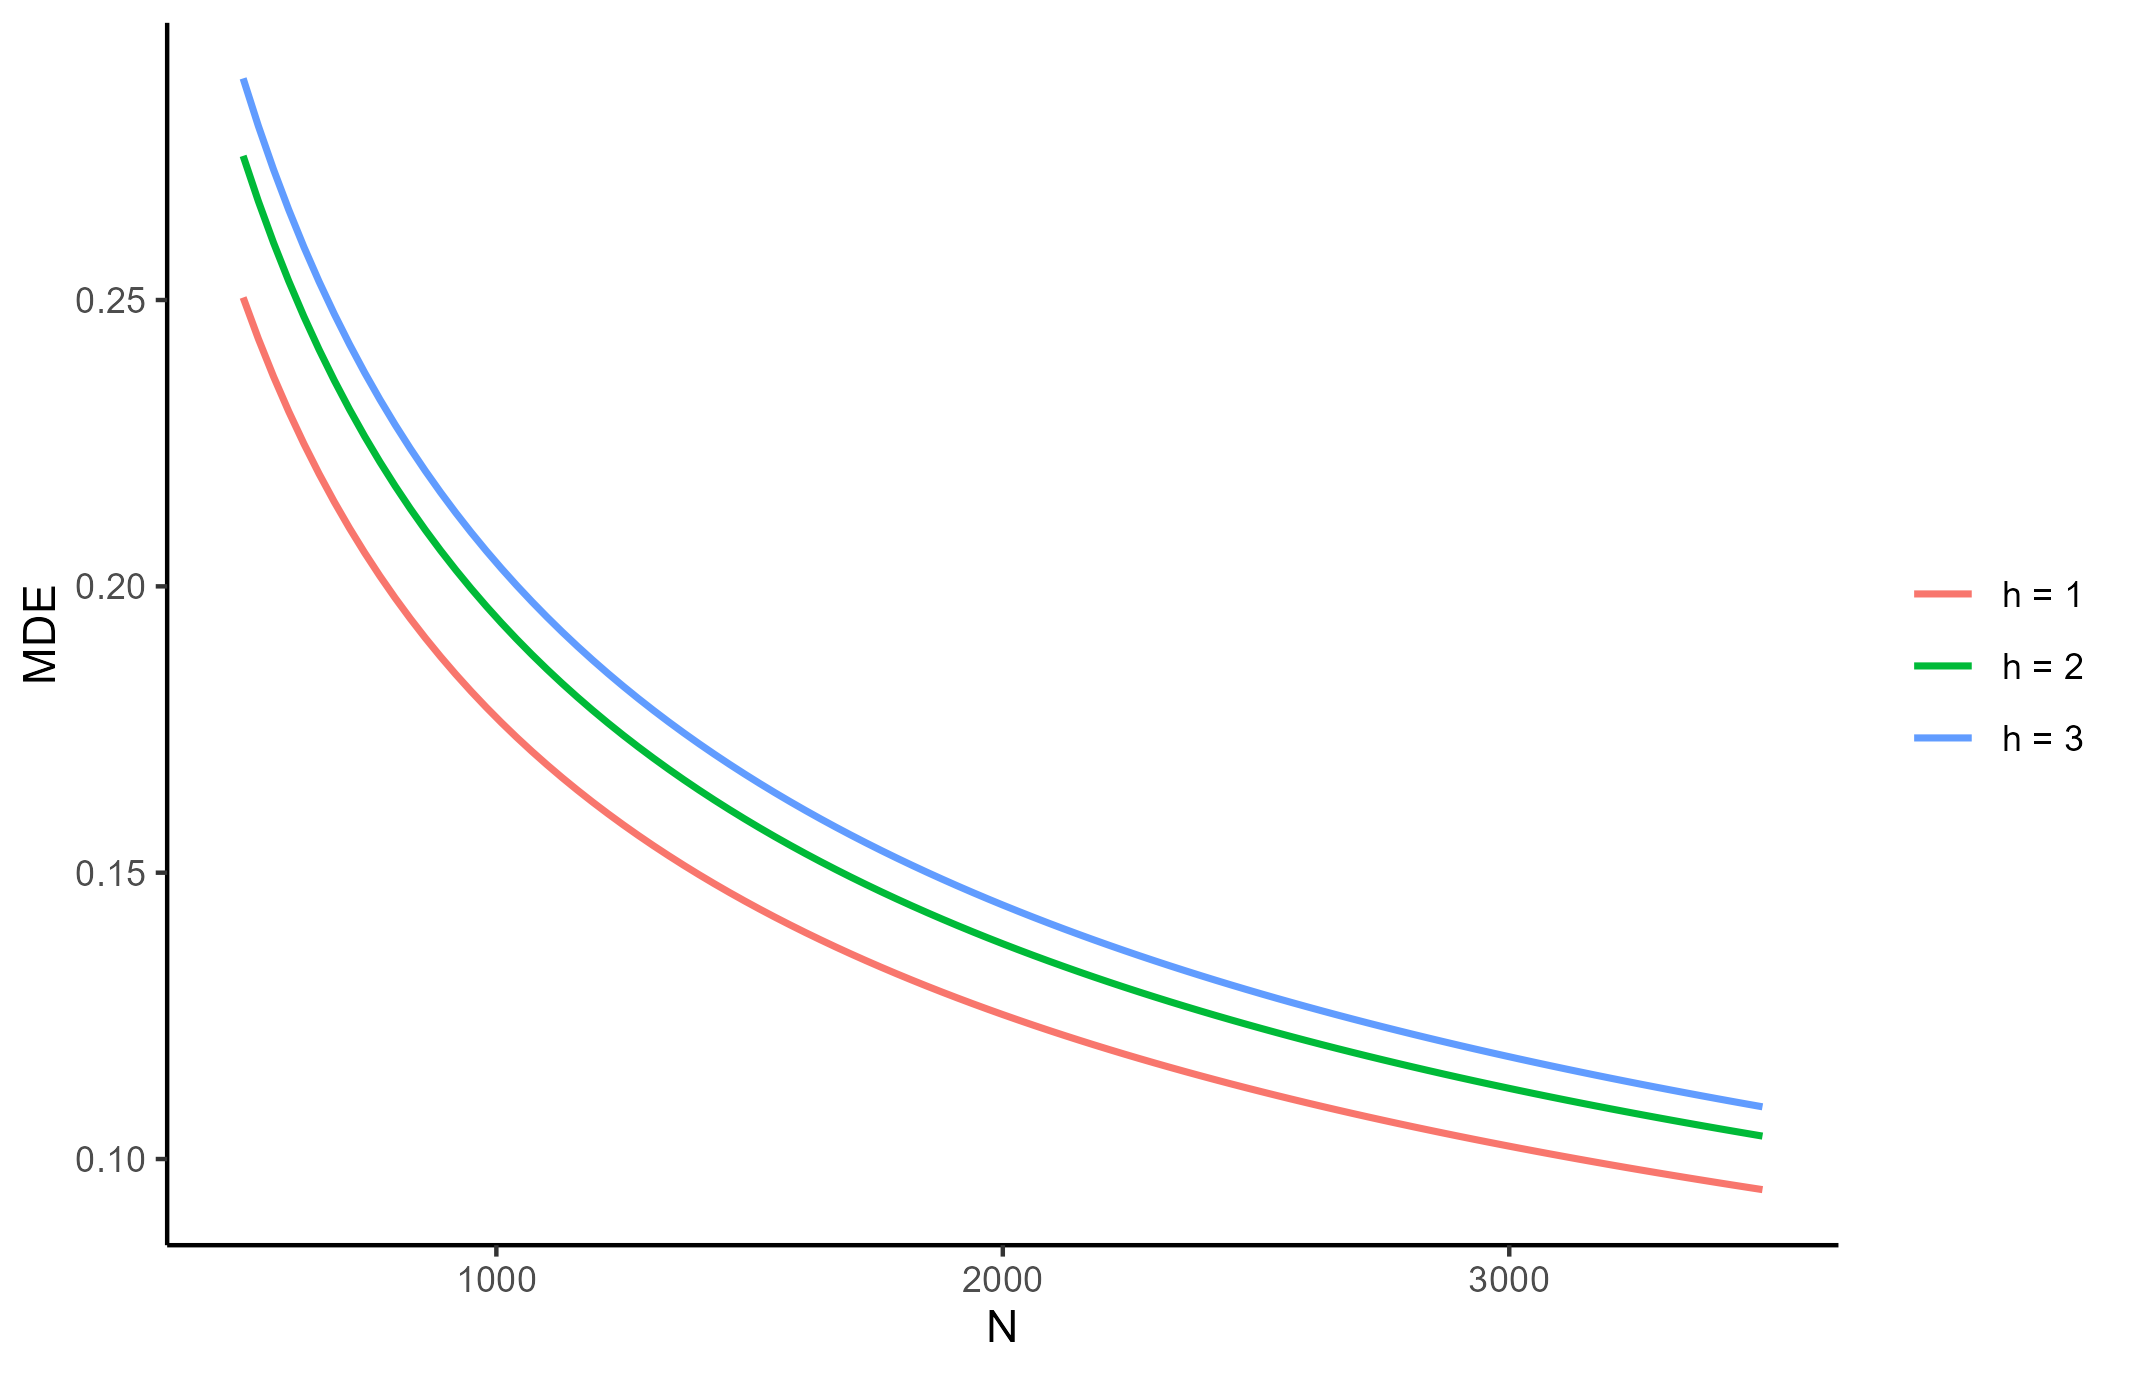
\includegraphics[width=0.8\linewidth]{Figuras/mde_h.png}
    \caption{Gráfico do MDE em termos de desvio padrão variando o tamanho da amostra de 500 a 3500 para diferentes valores de hipóteses a serem testadas conjuntamente.}
    \label{fig:mde_h}
\end{figure}